\documentclass{article}
\usepackage[utf8]{inputenc}
\usepackage{graphicx}
\graphicspath{ {images/} }
\usepackage[letterpaper, portrait, margin=1.7in]{geometry}
\usepackage{wrapfig}

\renewcommand{\baselinestretch}{2}

\title{Color In A Digital World}
\author{Kesley Copley }
\date{December 2015}

\begin{document}

\maketitle

\begin{abstract}
Color is an experience relative to the observer, and it means something different to everyone. In this paper, I go in depth into the perceptions of color. I talk about color spaces and color models and how color fits into the modern world completely taken over by technology. Color progresses much like technology does. I talk about the different aspects of color like saturation in relation to how we see it. I also discuss different species’ perceptions and abilities to see color and our own genetic deficiencies to be unable to see color. 
\end{abstract}

\section{Introduction}
\paragraph
\indent "Everything that you can see in the world around you presents itself to your eyes only as an arrangement of patches of different colors," said by John Ruskin, an English writer and artist. As an artist, I deal with color everyday. Whether it's actually mixing colors and painting or seeing a leaf that fell from a tree and admiring the shade of yellow it's turned into as summer progressed to autumn, I constantly think about color. I've worked with Photoshop and digitally recreated images. I've used an antique Polaroid camera and seen films in technicolor that were remade to be in HD digital. I see and utilize color thousands of times everyday and still, I don't appreciate it as much I could. Chemists, physicists, and computer scientists understand color much differently that I do, and in this paper, I will discuss aspects of color beyond that of art and sensation. First, I will discuss the broad understanding of color. I will then introduce digital color spaces and color models and applications for those. There are many things that affect the color we actually perceive, and I talk about those and the effect they have. Lastly, I will bring up color blindness and the different perceptions of color based on gender and species. 

\section{What is color?}
\paragraph
\indent Color is a fundamental part of the human experience. Everyday the human brain receives a barrage of information about the world and has to make sense of the input. That sensory data comes from the skin, the eyes, the ears, the nose, and the tongue. In the case of seeing color, light is reflected off an object. Its wavelengths are then picked up by the color receptors in the eyes. Cone cells, like in Figure 1, in the eyes detect red, blue, and green light. The visual information travels to the brain through the optic nerve. It is then interpreted by the brain and stored for later reference. The average human being does not know how much light is being reflected when they look at a firetruck or a school bus. They see what they have been taught to understand is red and yellow. And without the parts of the eyes that distinguish saturation and color, literally everything would be different. Without color, humans would not know that a banana has passed its ripe period or when a pepper is ready to pick.
\begin{wrapfigure}{l}{0.2\textwidth}
    \centering
    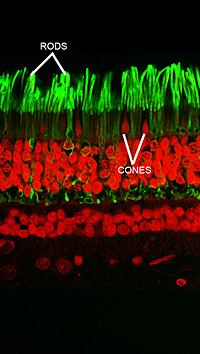
\includegraphics[width=0.2\textwidth]{cones}
    \caption{The rods and cones inside the human eye}
    \centering
\end{wrapfigure}
 Humans would not be able to tell the difference between a venomous snake or one that’s harmless. Not only is color important to humans, but to other animals as well. Hummingbirds, for example, are attracted to the color red because that is the color they associate with flowers, so many hummingbird feeders are red to attract more of the birds. Also, the male hummingbirds have brightly colored necks to get the attention of a possible mate, while females have more muted colors to act as a camouflage from predators.
\paragraph
\indent Color is a tool, a way of expressing feeling and generating emotion. Color is a sensational experience that will change the way people see something. Color is specifically artificial and pigmentation; it is created and prone to change. I can do anything I want with color. With color, I can cause anxiety and curiosity, happiness and hopelessness. In art class, kids are taught that red, blue, and yellow are the primary colors. Mixing the primary colors would result in the secondary colors of violet, green, and orange. Art has its secrets as well. To make brown, you mix complementary colors. To make a color a darker shade, you add black, and to achieve a lighter tint, you add white. A drop of black in a cup of yellow will make the most unappetizing color anyone has ever seen. One splash of color in a black and white painting will say more than a ten page paper. Color is not only a tool, though, because color itself is a creation. It is a very satisfying thing when the colors finally mix right to paint the correct skin shade needed for a portrait. To an artist, it is not wavelengths and reflected light on the paper. It is not just sensory input for the brain to decipher. To see color as an artist sees it, is a gift because there is nothing more personal than their perception of color.

\section{The world of digital color}
\paragraph
\indent In the modern age of technology, everyone in the United States, and in most other countries, look at a screen at least once a day, maybe more. People carry their phones, tablets, and PC’s around with them everywhere they go. Billboards are digitized, and television screens have been placed everywhere in stores, restaurants, and on the streets. Technology has become so integral to an average person’s daily life to the point where they could not normally function without a digital screen. But what are we actually looking at when we browse on our phones? Much like the artist's color palette, the digital color palette can be altered and made to have a certain effect. Like the human eyes, a computer generates three colors of light: red, blue, and green. In each pixel on a computer screen, there are three phosphors. They emit red, green, and blue light when struck by electron beams. The screen appears black when no electrons strike the phosphors, and the screen appears white when all three phosphors are struck at a high intensity.
\begin{figure}[h]
\centering
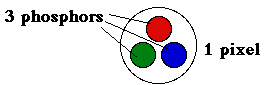
\includegraphics[scale=.7]{phosphors}
\caption{A pixel with the three phosphors that determine what color will show up on screen.}
\centering
\end{figure}

\section{What is color space?}
\paragraph
\indent The RGB color model is an example of an additive color model. In this model, the three additive primary colors are red, green, and blue. This relates to the eye's capabilities to detect red, blue, and green light. Color space is another word for a color model. Color space mathematically and visually represents a range of usually three color components using a coordinate system. Color spaces are typically helpful when trying to understand the color capabilities of a device or a digital file. Color can be represented using the Cartesian coordinate system, or X, Y, Z. When there is no red, blue, or green light, the point would remain at the origin emitting black at (0,0,0). The presence of all three primary colors would emit white light at the point (1,1,1). 
\begin{figure}[h]
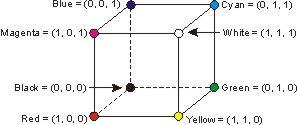
\includegraphics[scale=2]{color_cube}
\centering
\caption{RGB color model represented three-dimensionally using Cartesian coordinates.}
\centering
\end{figure}
\newline
\indent The RGB color model, shown in Figure 4, is an additive color model, where the primary colors are red, green, and blue. The secondary colors are cyan or a mixture of blue and green, magenta or red and blue, and yellow or red and green. The combination of the three primary additive colors produces white. Another model, that is used in color printing, is the CMY or CMYK model, shown in Figure 5. This is a subtractive color model where the name stands for cyan, magenta, yellow, and black. The RGB model is good for digital images and color matching, but when printing, the three subtractive primary colors filter out red, green, and blue and make the pigmentation necessary to recreate images on paper.

\begin{figure}[h]
\centering
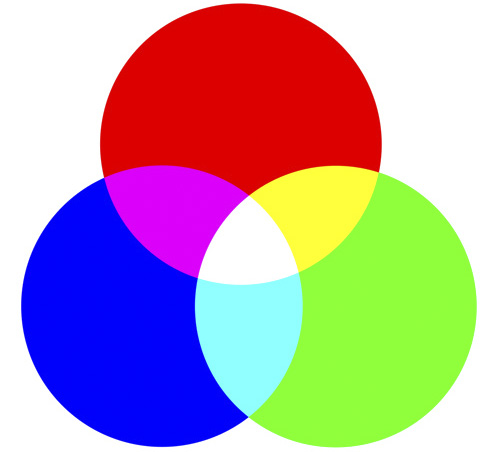
\includegraphics[scale=0.2]{color_space}
\caption{This is the average RGB color model representing the primary and secondary additive colors.}
\centering
\end{figure}
\begin{figure}[h]
\centering
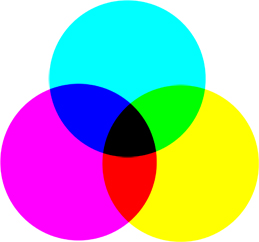
\includegraphics[scale=.4]{cmyk}
\caption{This is the CMYK color model including the subtractive primary colors.}
\centering
\end{figure}
\newline
\section{Applications of color space}
\paragraph
\indent One of the most popular applications for color spaces is color photography. At first, to capture a photograph, the photographer would have to use paper treated with a light-sensitive substance like silver nitrite or silver chloride. The images that were produced were too faint or came out as negatives. The quality of the image would be affected by the exposure time and the resin used on the paper. Reproducing images in color was the goal for a long time, and in 1848, a French physicist named Alexandre-Edmond Becquerel discovered a way to make color images; however, the techniques were impractical due to long exposure times and short-lasting color, so it was rarely done. James Clerk Maxwell, known for his research in electromagnetism, showed the first lasting color photograph using red, green, and blue colored filters, and all three were projected and superimposed on the original image.
\begin{wrapfigure}{l}{0.3\textwidth}
    \centering
    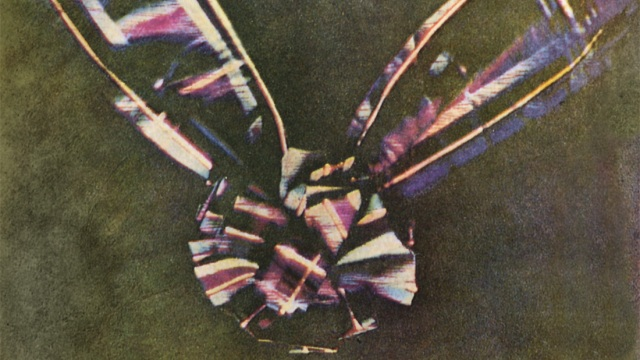
\includegraphics[width=0.3\textwidth]{maxwell}
    \caption{The first color image using color filters.}
    \centering
\end{wrapfigure}
This is known as the "color separation" method. Figure 6 is the image Maxwell presented of a tartan ribbon using color filters and transparent prints \cite{maxwell}. Another application of color that is a constant in our daily lives is film or video recording. That, much like still images, has a long history of trying to reproduce clear color reproductions. Technicolor film started with a two-color additive system recording the blue-green and red images through a single lens \cite{technicolor}. Technicolor cameras made another leap forward when people started using a subtractive two-color system. A subtractive system carries the color information within the images itself, so there is no need for filters. This means that colors could be reproduced more accurately. The negative of an image includes both red and blue-green information. The two different images were then produced and cemented together to create the final full color image. The first digital camera was created in 1975 by Steve Sasson at Kodak. The camera was eight pounds and recorded in 0.01 megapixels on a cassette tape. The photograph took 23 seconds to capture in black and white \cite{digital_camera}. A 1990 Dycam model was the first commercially-produced digital camera. It digitally stored pictures, used a CCD image sensor, and connected directly to a computer. Photography has come a long way to being able to capture images on a cell phone, being able to record events live and broadcast them on the Internet, and altering digital photographs to the point where the human eye would not be able to tell that they were altered. 

\section{Other factors of color}
\paragraph
\indent There are many other factors involved in dealing with color. One is the hue, which is essentially interchangeable with color. The hue of navy, for example, is blue. There are two ways to describe a color. The first is using the RGB model. The amount of red, green, and blue can be measured and be described that way. The other way to describe a color is through hue, saturation, and brightness. On the color wheel, the hue specifies the specific tone of color. The saturation can be changed by adding gray to the color. High saturation or vivid color has no gray, and a gray tone has no saturation. Lastly, brightness is affected by how much white is added to the color.  No brightness or completely black to full brightness which is completely white. This spectrum includes every shade and tint of a specific color. 
\begin{wrapfigure}{l}{0.5\textwidth}
    \centering
    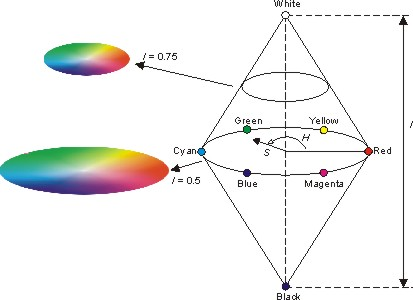
\includegraphics[width=0.5\textwidth]{hsi}
    \caption{The HSI color model describing the different levels of hue, saturation, and intensity.}
    \centering
\end{wrapfigure}
Mostly, colors are thought to be more pleasing to they eye at a lower saturation, so a lot of wall paints have been treated with gray to lower the saturation level. The intensity of a color is another word for the saturation; it’s how vivid or dull the color is. The HSI color model, as shown in Figure 5, is an important model for image processing \cite{color_model}. We can digitally recreate an image by affecting the levels of intensity, hue, and saturation. One thing people do with smartphones is change the levels of saturation, brightness, and hue of their pictures making them brighter or more saturated to give them a more pleasing appeal. Isaac Newton performed experiments with light and color. He first explained the cause behind a rainbow using white light shining through a prism which experiences rarefaction and comes out as all the colors of the rainbow. Color was thought to be a mixture of light and dark, and Newton set out to prove that color was in the light itself. From these experiments, he created something known as a Hue circle. This was a primitive idea that became a tool for artists and is still incorporated into the modern color wheel.
\newline
\begin{figure}[h]
\centering
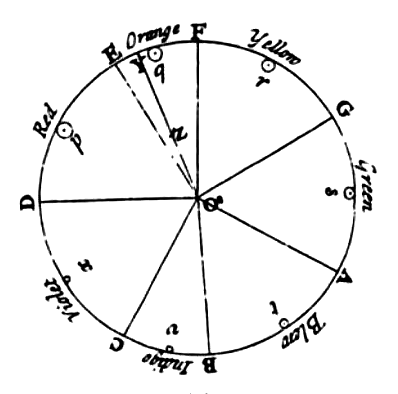
\includegraphics[scale=0.3]{newton}
\caption{Isaac Newton's Hue circle}
\centering
\end{figure}


\section{How we see color}
\paragraph
\indent Color, as I have discussed, is a visual perception. Color does not actually exist. Without the eyes to translate light into perceived color in the brain, then color would not actually be a reliable quality. How true is it that women see better than men? Why is it that when women see a paint color, it’s eggshell, but men genuinely see white and only white? In experiments done by Israel Abramov, women proved to be better at distinguishing subtle color gradients in the yellow-green part of the color spectrum. An object that looks orange to women will seem slightly more red to men due to the discovery that men need a slightly longer wavelength to see the same hue as women. Here is experimental proof that women see color at a finer level than men. In the experiment, Abramov also studied to see whether men and women see objects that are farther away differently. It was found that men could see details about objects that are farther away. A theory to explain this that isn’t close to being proven is that through biological evolution and adaptation, women have developed a finer detail in seeing color in order to spot ripe fruits while foraging. Men, on the other hand, adapted to seeing objects that are farther away for hunting purposes \cite{men_women}. This only a possible explanation for why this happens. 
\paragraph
\indent Humans have trichromatic vision. This means we have three different photopigments. A photopigment undergoes a chemical reaction when it absorbs light and depending the photopigment that is hit, that is the color that our brain perceives. They have individual sensitivities to certain wavelengths of light. Blue light or small wavelengths, green or medium wavelengths, and red or long wavelengths \cite{color_vision}. Humans are not the only species that can see color. Mantis shrimp have twelve color receptors meaning they should be able to see a multitude of colors that we wouldn’t even dream of. It was found this is not the case. The shrimp can detect a difference in wavelengths of about 25 nanometers apart while humans can detect differences four nanometers apart \cite{shrimp}. Cats can see color but lack the ability to see red very strongly. Dogs also see color; however, they see less than humans because they have less cones and rods \cite{dogs_cats}. Butterflies have a very wide range of vision. Some butterflies have pentachromatic visual system which means they can detect five wavelength peaks including ultraviolet light \cite{butterflies}.
\paragraph
\indent There is a lot of confusion associated with color blindness or color vision deficiency. Color blindness is hereditary, and about eight percent of men have red-green color blindness, while less than one percent of women have it. Color blindness is a mutated gene that is passed down from mother to child on the X chromosome, and because women have two X chromosomes, it less likely for women to be affected by the gene \cite{color_blind}. Color blindness can range in severity from almost normal color perception to complete color blindness. The most common form of color blindness is red-green color blindness where the person has no or limited function of the red cone or the green cone. A less rare type of color blindness is blue-yellow color blindness where the blue cone photopigments have been lost or have limited functionality. People with complete color don’t experience color at all with the clearness of their vision possibly affected as well. The most severe kind of color blindness is rod monochromacy or achromatopsia, where none of the cone cells have functional photopigments. People with this see the world in black, white, and shades of gray \cite{color_blind}. There is no cure or solution for color blindness; however, there is a new set of lenses named EnChroma lenses that enhance the intensity and saturation of colors in objects. 
\newline
\begin{figure}[h]
\centering
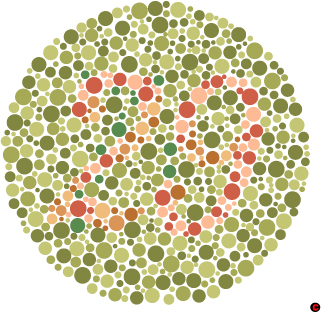
\includegraphics[scale=0.5]{testt}
\caption{An image used to determine whether a person has red-green color blindness, depending on whether they can see the number inside the circle.}
\centering
\end{figure}

\section{Conclusion}
\paragraph
\indent In this paper, color has been discussed at length. I have found that color will stand the test of time and continue to evolve and progress with technology. The human experience would not be as it is without our ability to see color. We can manipulate digital images to do whatever we want because of the color spaces that were modeled after the color receptors in our own eyes. A genetic deficiency that humans must deal with is color blindness. As of right now in 2015, there is no cure for color blindness, only a pair of lenses that slightly improve the mild cases. As technology continues to grow more sophisticated, so will our understanding of how to replicate and artificially create the cones and rods necessary to see colors to their full vibrancy.
\newpage
\bibliographystyle{unsrt}
\bibliography{references}
\end{document}